%%%%%%%%%%%%%%%%%%%%%%%%%%%%%%%%%%%%%%%%%
% Conceptual Group Report
%
% This template has been downloaded from:
% http://www.LaTeXTemplates.com
%
% With links assisting from
% https://guillaumeblanchet.medium.com/using-latex-in-visual-studio-code-on-windows-121032043dad
%
%%%%%%%%%%%%%%%%%%%%%%%%%%%%%%%%%%%%%%%%%

%----------------------------------------------------------------------------------------
%	PACKAGES AND OTHER DOCUMENT CONFIGURATIONS
%----------------------------------------------------------------------------------------

\documentclass[a4paper,11pt]{article}

%%%%%%%%%%%%%%%%%%%%%%%%%%%%%%%%%%%%%%%%%
% Arsclassica Article
% Structure Specification File
%
% This file has been downloaded from:
% http://www.LaTeXTemplates.com
%
% Original author:
% Lorenzo Pantieri (http://www.lorenzopantieri.net) with extensive modifications by:
% Vel (vel@latextemplates.com)
%
% License:
% CC BY-NC-SA 3.0 (http://creativecommons.org/licenses/by-nc-sa/3.0/)
%
%%%%%%%%%%%%%%%%%%%%%%%%%%%%%%%%%%%%%%%%%

%----------------------------------------------------------------------------------------
%	REQUIRED PACKAGES
%----------------------------------------------------------------------------------------

% \usepackage[
% nochapters, % Turn off chapters since this is an article        
% % beramono, % Use the Bera Mono font for monospaced text (\texttt)
% eulermath,% Use the Euler font for mathematics
% pdfspacing, % Makes use of pdftex’ letter spacing capabilities via the microtype package
% dottedtoc, % Dotted lines leading to the page numbers in the table of contents
% ]{} % The layout is based on the Classic Thesis style

% \usepackage{showframe}

\usepackage[a4paper, margin=1in]{geometry}

% \usepackage{arsclassica} % Modifies the Classic Thesis package

\usepackage[T1]{fontenc} % Use 8-bit encoding that has 256 glyphs

\usepackage{titling} % To control the title
\setlength{\droptitle}{-4.5em}   % This is your set screw

\usepackage[utf8]{inputenc} % Required for including letters with accents

\usepackage{fancyhdr} % Allows for the inclusion of fancy headers

\usepackage{graphicx} % Required for including images
\graphicspath{{Figures/}} % Set the default folder for images

\usepackage{glossaries} % Allows for a nice list of glossaries

\usepackage{enumitem} % Required for manipulating the whitespace between and within lists

\usepackage{lipsum} % Used for inserting dummy 'Lorem ipsum' text into the template

\usepackage{subfig} % Required for creating figures with multiple parts (subfigures)

\usepackage{amsmath,amssymb,amsthm} % For including math equations, theorems, symbols, etc

\usepackage{varioref} % More descriptive referencing

\usepackage{hyperref}

\usepackage{gensymb}

\usepackage{tabularx}

\usepackage{appendix}

%----------------------------------------------------------------------------------------
%	HEADING STYLES
%---------------------------------------------------------------------------------------
\pagestyle{fancy}
\fancyhf{}
\setlength{\headheight}{14pt}
\fancyhead[R]{\lowercase{\thetitle}} % TODO MAKE LOWER CASE
\fancyhead[L]{\thepage}

%----------------------------------------------------------------------------------------
%	THEOREM STYLES
%---------------------------------------------------------------------------------------

\theoremstyle{definition} % Define theorem styles here based on the definition style (used for definitions and examples)
\newtheorem{definition}{Definition}

\theoremstyle{plain} % Define theorem styles here based on the plain style (used for theorems, lemmas, propositions)
\newtheorem{theorem}{Theorem}

\theoremstyle{remark} % Define theorem styles here based on the remark style (used for remarks and notes)

%----------------------------------------------------------------------------------------
%	HYPERLINKS
%---------------------------------------------------------------------------------------

% \hypersetup{
% %draft, % Uncomment to remove all links (useful for printing in black and white)
% colorlinks=true, breaklinks=true, bookmarks=true,bookmarksnumbered,
% urlcolor=webbrown, linkcolor=RoyalBlue, citecolor=webgreen, % Link colors
% pdftitle={}, % PDF title
% pdfauthor={\textcopyright}, % PDF Author
% pdfsubject={}, % PDF Subject
% pdfkeywords={}, % PDF Keywords
% pdfcreator={pdfLaTeX}, % PDF Creator
% pdfproducer={LaTeX with hyperref and ClassicThesis} % PDF producer
% }


% Helpful links for latex
% https://guillaumeblanchet.medium.com/using-latex-in-visual-studio-code-on-windows-121032043dad

\title{Boosting System for Fuel Cell vehicles}

\author{Galen Korosec, Gigi Wong, Ryan Jessop, Shreyan Mandal \& Yaoquan Tang}

% \date{2020–01–13}

\begin{document}

\maketitle

\section*{Abstract}

The report details the initial development stage of a hydrogen fuel cell testing rig. A hydrogen fuel cell is a type of power cell capable of converting the chemical energy of hydrogen into electricity. Its method of operation utilises hydrogen and air/oxygen particles and the testing rig is planned to be utilised to test how a hydrogen fuel cell performs for efficiency when provided with varying pressure ratios of the incoming gases. It is proposed that the development of the testing rig will involve numerous subsystems of the testing rig which are air intake and boosting, heat management systems, water management systems and system regulation of gas characteristics. It is noted that interest in fuel cell performance has grown due to the recent political pushes toward greater development of more environmentally conscious methods of transport.

\tableofcontents

\section*{Abbreviations}

%\begin{center}
\begin{tabular}{ l l }
    \textbf{FCEV} & Fuel Cell Electric Vehicle \\
    \textbf{PEM} & Polymer Electrolyte Membrane \\
    \textbf{LT-PEM} & Low-temperature Polymer Electrolyte Membrane \\
    \textbf{HMS} & Heat Management System \\
\end{tabular}
%\end{center}

\section{Introduction}

Fuel cell vehicles are gaining increased attention for authorities and industries to align with the Carbon Net-Zero target by 2050. To achieve the goal of limiting global temperatures rise to 1.5 °C, global demand for hydrogen fuel is expected to sixfold to 530 million tonnes in 2050; By then, 90\% of road transport should be powered by renewable energy, with 37\% being hydrogen-fuelled vehicles \cite{IEA2021netzero}. The Hydrogen Roadmap Europe has projected that there will be 3.7 million fuel cell vehicles on the road by 2030 \cite{FCHJU2019roadmap}, implying that the figure in 2050 could go as high as 9.8 million vehicles. 

Despite the rigorous forecast in demand for hydrogen-fuelled vehicles, there are various difficulties in promoting hydrogen-fuelled vehicles, mainly due to the low power converting efficiency [DOE, 2006]. This project intends to increase power efficiency and explore the feasibility of developing a boosting system for hydrogen Fuel Cell Vehicles (FCV). A test rig is also designed to measure the booster efficiency. 

This report first addresses the primary and secondary objectives of the project; second, it explains the background of the selection of system components, including the type of fuel cell and forms of hydrogen; finally, it goes into the overview of the proposed solution, which comprehends by the complete picture of the entire system and the five supporting subsystems.

\section{Objectives}

The subject is researching the booster system that increases the efficiency of the FCVs. As mentioned, a test rig will be designed. Data will be collected in the test rig, which will be used for quantifying measurement and simulation to prove feasibility. This should contain a variety of sensors responsible for measuring temperature, pressure, humidity, flow, etc. The data collected will be input into the designed system console for analysis. At the same time, appropriate electronic load devices will be used, which will be responsible for measuring the output power of the fuel cell.

Theoretically, the higher the reaction pressure, the higher the fuel cell's performance. Therefore, the control variable method is adopted. First, experiments are carried out with hydrogen under constant pressure, and the power of the battery system is tested by controlling the pressure of the air in which the reaction is carried out. Then, experiments are carried out with air under constant pressure, and the power of the battery system is tested by controlling the pressure of hydrogen gas. At the same time, factors such as temperature and humidity that may affect the experimental results should also be considered. Finally, the project will identify the maximum power generation efficiency that can be safely achieved under experimental conditions.

\section{Background}


In 2019 27\% of UK emissions came from road transport \cite{waite2019emissions}. To reach the UK's and global emissions targets, alternatives to the internal combustion engine need to be considered. Fuel cell electric vehicles (FCEVs) provide an attractive option \cite{yoshida2015toyota}. A fuel cell vehicle uses hydrogen as its fuel source. Electricity is generated via a chemical reaction between oxygen and hydrogen to create water; as can be seen in equation \ref{eq:pemChem}. This electricity is stored in a battery and uses an electric motor to move. One of the main advantages of an FCEV over a traditional battery-powered electric vehicle (BEV) is the refuelling time. A typical electric car such as the Nissan LEAF takes 7 hours 30 minutes to fully recharge from empty, giving a range of 168 miles \cite{Nissan2022Elec}. Compared to the 3 minutes of an FCEV like the Toyota Mirai \cite{yoshida2015toyota}. 

\begin{equation} \label{eq:pemChem}
    2H_{2} + O_2 \rightarrow 2H_{2}O + energy
\end{equation}

While the exact reaction differs between fuel cell types, the general process can be seen in the diagram\ref{fig:fuelCellBasic} \cite{Mark2003SolidOxide}. The system is composed of an anode, a cathode, an electrolyte and the load or external circuit. At the anode, hydrogen is oxidised into protons and electrons. At the cathode, oxygen is ionised, then depending on the electrolyte type, either the oxygen ions or the protons are transported over the electrolyte. At the same time, the electrons travel externally to provide electrical power \cite{Mark2003SolidOxide}.


\begin{figure}[h!] \label{fig:fuelCellBasic}
    \includegraphics[width=\textwidth]{fuelCellBasics.jpg}
    \caption{Diagram of the general operating principles of a fuel cell \cite{Mark2003SolidOxide}}
    \centering  
\end{figure}

Currently, there are three main types of fuel cells used in road vehicles, Polymer Electrolyte Membrane (PEM), Alkaline fuel cells (AFCs), and Phosphoric Acid fuel cells. A summary of each can be seen in table \ref{tab:fuelComparison}. PEM is used most in FCEVs. Its high usage is due to its low operating temperatures, quick start-up time and ability to use atmospheric air\cite{deloitte2020FuelCell}. However, it uses Platinum as a catalyst which increases its cost. AFCs operate similarly to PEMs. However, they use an alkaline electrolyte instead of an acid-based one used in the PEMs. The AFC electrolyte transports OH- ions from the cathode to the anode. Finally, there is Phosphoric acid fuel cells they have the potential to be incredibly efficient with results as high as 80-85\% when reclaiming the heat\cite{doe2006factsheet}; however without this additional system it is around 40\%. For these reasons the test rig was designed around the PEM.

\begin{table}[h!]
    \centering
    \begin{tabular}{|p{0.15\textwidth}||p{0.15\textwidth}|p{0.15\textwidth}|p{0.15\textwidth}|p{0.15\textwidth}|} %{|l||c|c|c|c|}
     \hline
     \multicolumn{5}{|c|}{Common fuel cell comparison} \\ 
     \hline
     Fuel Cell & Operating temperature & Catalyst type & Operating pressure & Electrical efficiency \\
     \hline\hline
     PEM & 50-100\degree C & Platinum & 3-4 bar & 50-60\% \\
     \hline
     AFC & 90-100\degree C & Nickle/Silver & 3-4 bar & 60-70\% \\
     \hline
     Phosphoric Acid & 150-200\degree C & Platinum & 7507 & 80-85\%(with combined heat and power) 40\% electric\\

    %  5 & 88 & 788 & 6344 \\ [1ex] 
     \hline
    \end{tabular}
    \caption{Table comparing different fuel cells}
    \label{tab:fuelComparison}
\end{table}

To improve the attractiveness of fuel cell vehicles, their efficiency needs to be improved. For PEM fuel cells, research has shown that controlling the incoming air pressure can increase the system efficiency \cite{hoeflinger2020air}. As the fuel cell technology improves, the boosting needs to be optimised; for this reason, a testing rig to assist with the investigation into the effects of boosting is beneficial. 

\section{Overview of Proposed solution}

\begin{figure}[h!] \label{fig:systemOverview}
    \includegraphics[width=\textwidth]{systemOverview.jpg}
    \caption{Diagram of the proposed test rig systems}
    \centering  
\end{figure}

\subsection{Air Intake and Boosting}
The air intake and boosting system will be the initial point where the ambient air at atmospheric pressure enters the system. The project brief aims to develop a testing rig for the fuel cell's power output at varying pressure ratios. This suggests that the boosting system needs to take the ambient air at atmospheric pressure and supply the system with the relevant ratios. The first stage in the project will be to determine a definitive range of pressure ratios that must be provided to the fuel cell to carry out the appropriate testing. This can be done by reading relevant literature on alternate methods of fuel cell tests on comparable fuel cell stack sizes and how the cells performed for these pressure ratios. For example, the study on the optimal pressure ratios of a PEM fuel cell\cite{hoeflinger2020air} indicated that the tested pressure ratios were between 1.0 and 2.2. A further review of multiple studies into the relevant fuel cells will show the necessary ratios.

In terms of designing the boosting system to provide a variable pressure ratio, the stages described in figure \ref{fig:airIntakeSys} are planned to regulate the values of pressure and the flow speed entering the concurrent subsystems. The ambient air temperature will also impact these values and the work required of the compressor. The Steady Flow Energy equation as seen in equation \ref{eq:rateOfHeatAdded} can be utilised to determine the values from the compressor to the intake receiver when consulting the operating power of the compressor's impeller. Here the values of $\dot{Q}$ represents the rate of heat added to the system to $\dot{W_{ext}}$, the rate of work done. The values for $\dot{m}$, mass flow rate of air in the compressor, $h_n$, enthalpy entering or leaving the system, $V_n$, speed of the air and $z_n$, the height at which the air enters or leaves the system, will be explored in the following works to describe how they can be found (note that $g$ describes acceleration due to gravity). This will the bassline amount power needed to operate the compressor, which will then need more to account for losses. Note that mass air flow valves and pressure gauges will be utilised in the subsystem to provide these necessary values. 

\begin{figure}[h]
    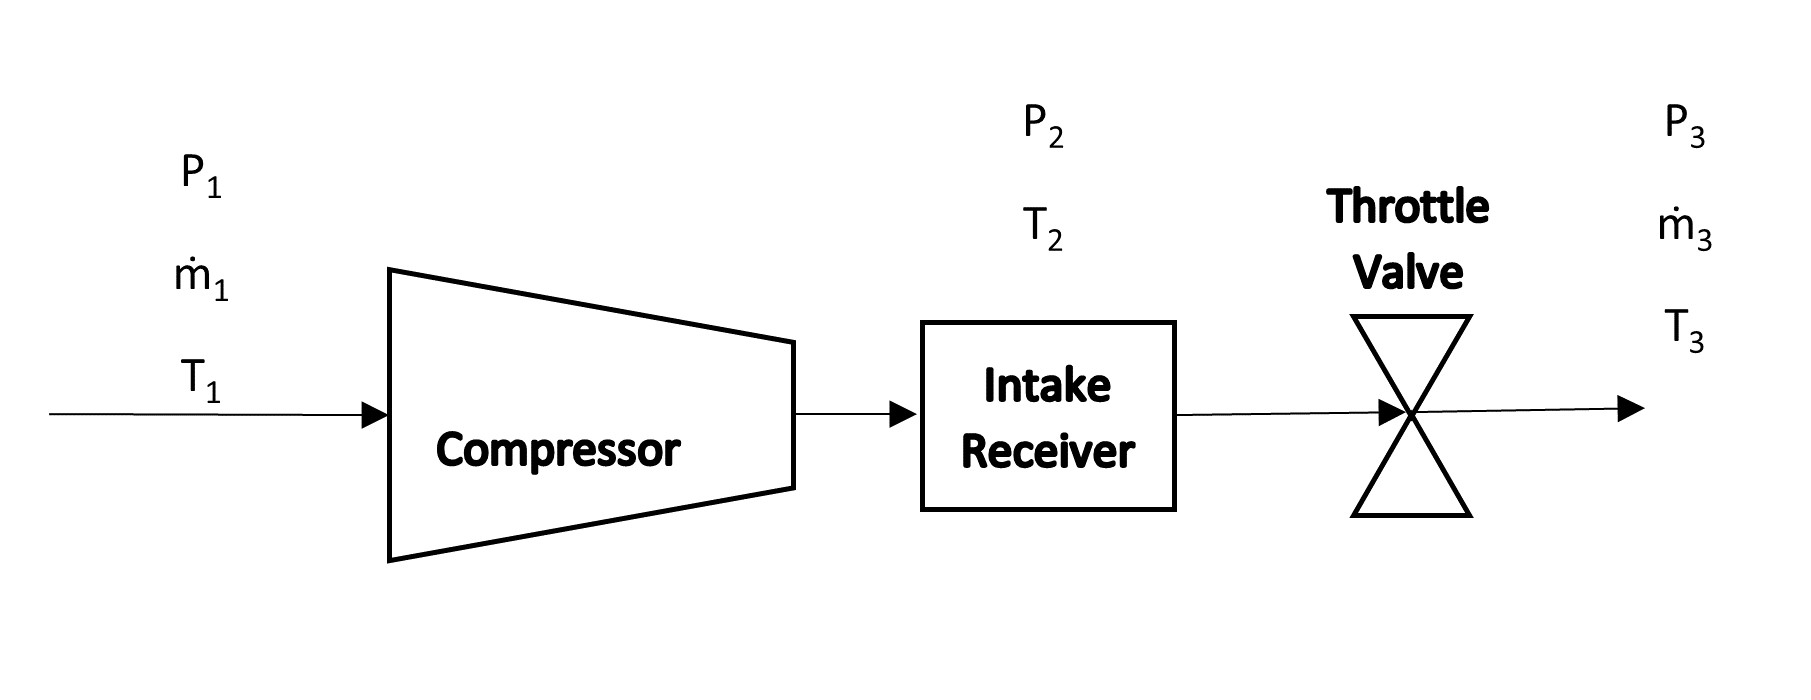
\includegraphics[width=\textwidth]{air intake system diagram.jpg}
    \caption{Diagram of the proposed test rig systems}
    \centering  
\end{figure}\label{fig:airIntakeSys}

\begin{figure}[h]
\begin{equation} 
    E=mc^2
\end{equation}
\caption{Steady Flow Energy equation}
\end{figure}\label{eq:rateOfHeatAdded}

The option to examine the effect of directly injecting oxygen into this system will be implemented. Here, the studies into relevant literature can also provide input on the impact of different levels of oxygen percentages entering the fuel cell. As part of investigating this option, the values of oxygen percentages in the incoming air will need to be kept track of. Further, the input location of such oxygen will need to be determined in conjunction with the other systems.  

\subsection{Heat Management}
Other subsystems are also vital in supporting the entire boosting system and the compressor. Heat Management is essential to maintain the system thermal and energy stability to withstand different environmental conditions. Steady-state operation of the fuel cell stack is critical to ensure maximum power output efficiency.  

The heat exchange mechanism of fuel cells involves two parts, heating and cooling. The LT-PEM fuel cell needs to be maintained at thermal equilibrium at 60-80\degree C throughout the operation for maximum efficiency. The hydrogen and oxygen need to be heated to the same temperature when entering the fuel cell stack. On the other hand, a cooling system is necessary to remove extra heat generated during the fuel cell reaction. Four cooling strategies are commonly used in fuel cell vehicles (as shown in Table 1). For a typical FCEV with 100kW power, edge cooling or heat spreader is insufficient; air flow cooling cannot be made efficient either without reducing the fuel cell reaction rate [Wen, 2011]. Phase change cooling is generally desirable but external coolant is required for vaporization cooling. Thus liquid cooling is most widely adopted on high power FCS for its strong cooling capability [Nguyen, 2020].  In this design, liquid cooling is selected as it allows recovering up to 36\% of energy from waste heat (Figure x) by combining with output water as coolant. This approach increases the system's overall power efficiency from recovering excess heat energy and up-cycles the water output as a coolant and humidifier for the gases. 

\newpage

%----------------------------------------------------------------------------------------
%	BIBLIOGRAPHY
%----------------------------------------------------------------------------------------

% \renewcommand{\refname}{\spacedlowsmallcaps{References}} % For modifying the bibliography heading

\bibliographystyle{IEEEtran}

\bibliography{references_galen,references_gigi} % The file containing the bibliography

%----------------------------------------------------------------------------------------


\end{document}